% ============================================================
% activity_diagram.tex
% Diagrama de actividades UML — "Registrar pedido" (P2)
% ISR-401 — Prueba Práctica Unidad IV
% ============================================================
% Este archivo puede compilarse de forma independiente o
% incluirse desde main.tex con % ============================================================
% activity_diagram.tex
% Diagrama de actividades UML — "Registrar pedido" (P2)
% ISR-401 — Prueba Práctica Unidad IV
% ============================================================
% Este archivo puede compilarse de forma independiente o
% incluirse desde main.tex con % ============================================================
% activity_diagram.tex
% Diagrama de actividades UML — "Registrar pedido" (P2)
% ISR-401 — Prueba Práctica Unidad IV
% ============================================================
% Este archivo puede compilarse de forma independiente o
% incluirse desde main.tex con % ============================================================
% activity_diagram.tex
% Diagrama de actividades UML — "Registrar pedido" (P2)
% ISR-401 — Prueba Práctica Unidad IV
% ============================================================
% Este archivo puede compilarse de forma independiente o
% incluirse desde main.tex con \input{diagramas/activity_diagram}
% ============================================================

\documentclass[tikz,border=10pt]{standalone}
\usepackage{tikz}
\usetikzlibrary{shapes.geometric, positioning, arrows.meta}

\begin{document}
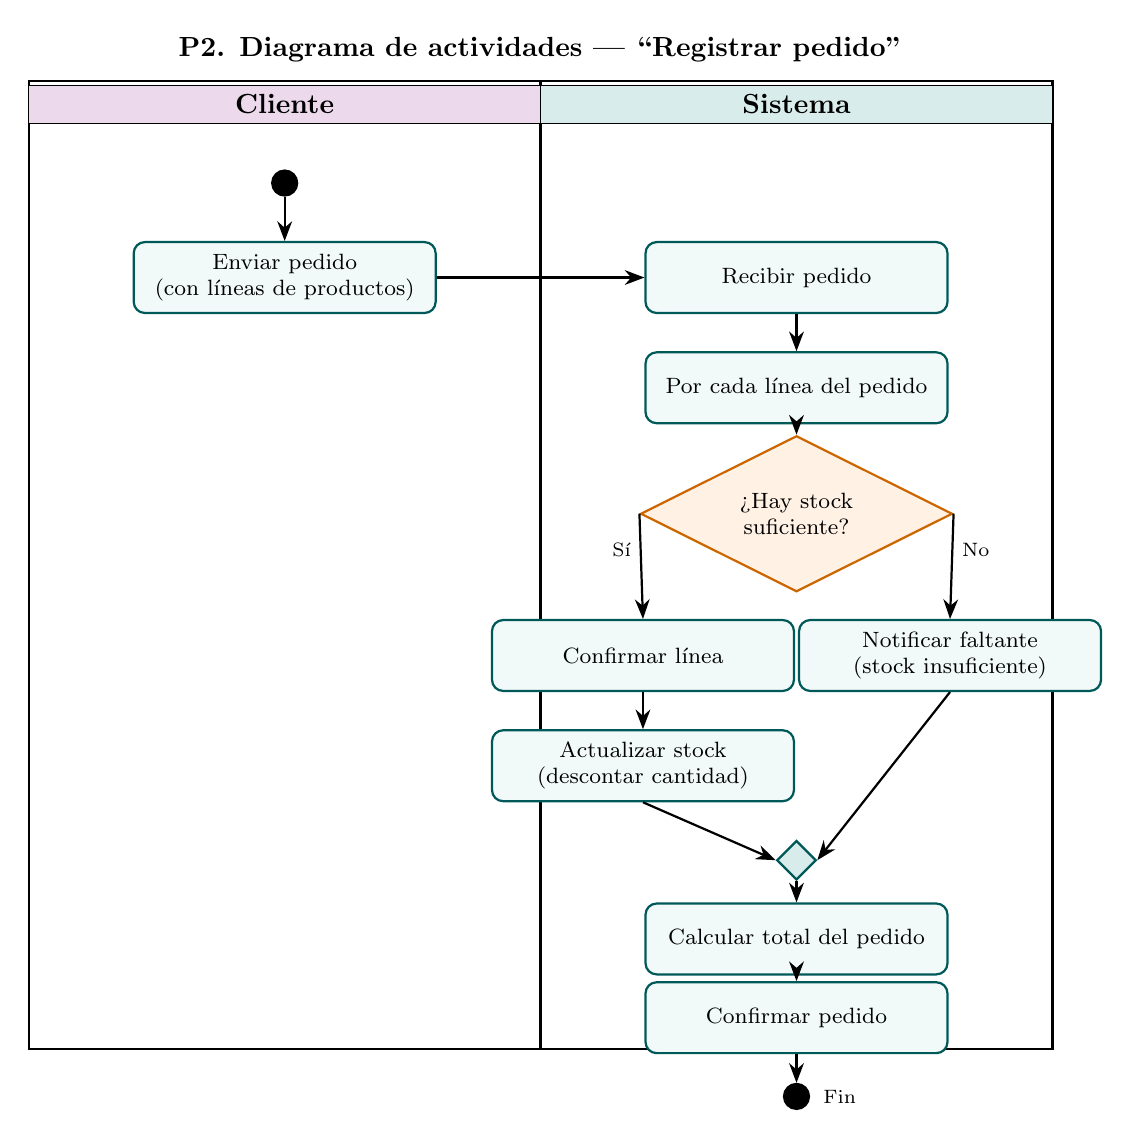
\begin{tikzpicture}[
    action/.style={rectangle, rounded corners, draw=teal!70!black, thick,
        fill=teal!5, text width=3.6cm, align=center, minimum height=0.9cm, font=\footnotesize},
    decision/.style={diamond, draw=orange!80!black, thick, fill=orange!10,
        aspect=2, text width=2.2cm, align=center, font=\footnotesize},
    merge/.style={diamond, draw=teal!70!black, thick, fill=teal!15,
        minimum width=0.5cm, minimum height=0.5cm},
    initial/.style={circle, draw=black, fill=black, minimum size=0.3cm},
    final/.style={circle, draw=black, fill=white, minimum size=0.4cm},
    finaldot/.style={circle, draw=black, fill=black, minimum size=0.2cm},
    swimlane/.style={draw=black, thick, minimum width=6.5cm},
    every edge/.style={draw, -{Stealth[length=2.5mm]}, thick},
    lbl/.style={font=\scriptsize}
]

% --- Título ---
\node[font=\bfseries] at (6.5,12.7) {P2. Diagrama de actividades --- ``Registrar pedido''};

% --- Carriles (swimlanes) ---
\draw[thick] (0,0) rectangle (6.5,12.3);
\draw[thick] (6.5,0) rectangle (13,12.3);
\draw[very thick] (6.5,0) -- (6.5,12.3);

\node[font=\bfseries, fill=violet!15, minimum width=6.5cm, draw] at (3.25,12) {Cliente};
\node[font=\bfseries, fill=teal!15, minimum width=6.5cm, draw] at (9.75,12) {Sistema};

% --- Carril Cliente ---
\node[initial] (ini) at (3.25,11) {};
\node[action] (enviar) at (3.25,9.8) {Enviar pedido\\(con líneas de productos)};

% --- Carril Sistema ---
\node[action] (recibir) at (9.75,9.8) {Recibir pedido};
\node[action] (porcada) at (9.75,8.4) {Por cada línea del pedido};
\node[decision] (hay) at (9.75,6.8) {¿Hay stock suficiente?};

\node[action] (confirmarLinea) at (7.8,5.0) {Confirmar línea};
\node[action] (notificar) at (11.7,5.0) {Notificar faltante\\(stock insuficiente)};

\node[action] (actualizar) at (7.8,3.6) {Actualizar stock\\(descontar cantidad)};

\node[merge] (union) at (9.75,2.4) {};

\node[action] (total) at (9.75,1.4) {Calcular total del pedido};
\node[action] (confirmarPedido) at (9.75,0.4) {Confirmar pedido};

\node[finaldot] (fin) at (9.75,-0.6) {};
\node[lbl] at (10.3,-0.6) {Fin};

% --- Flujo Cliente -> Sistema ---
\draw[-{Stealth[length=2.5mm]}, thick] (ini) -- (enviar);
\draw[-{Stealth[length=2.5mm]}, thick] (enviar.east) -- (recibir.west);

% --- Flujo Sistema ---
\draw[-{Stealth[length=2.5mm]}, thick] (recibir) -- (porcada);
\draw[-{Stealth[length=2.5mm]}, thick] (porcada) -- (hay);

\draw[-{Stealth[length=2.5mm]}, thick] (hay.west) -- (confirmarLinea.north) node[lbl, midway, above left] {Sí};
\draw[-{Stealth[length=2.5mm]}, thick] (hay.east) -- (notificar.north) node[lbl, midway, above right] {No};

\draw[-{Stealth[length=2.5mm]}, thick] (confirmarLinea) -- (actualizar);
\draw[-{Stealth[length=2.5mm]}, thick] (actualizar.south) -- (union.west);
\draw[-{Stealth[length=2.5mm]}, thick] (notificar.south) -- (union.east);

\draw[-{Stealth[length=2.5mm]}, thick] (union) -- (total);
\draw[-{Stealth[length=2.5mm]}, thick] (total) -- (confirmarPedido);
\draw[-{Stealth[length=2.5mm]}, thick] (confirmarPedido) -- (fin);

\end{tikzpicture}
\end{document}

% ============================================================

\documentclass[tikz,border=10pt]{standalone}
\usepackage{tikz}
\usetikzlibrary{shapes.geometric, positioning, arrows.meta}

\begin{document}
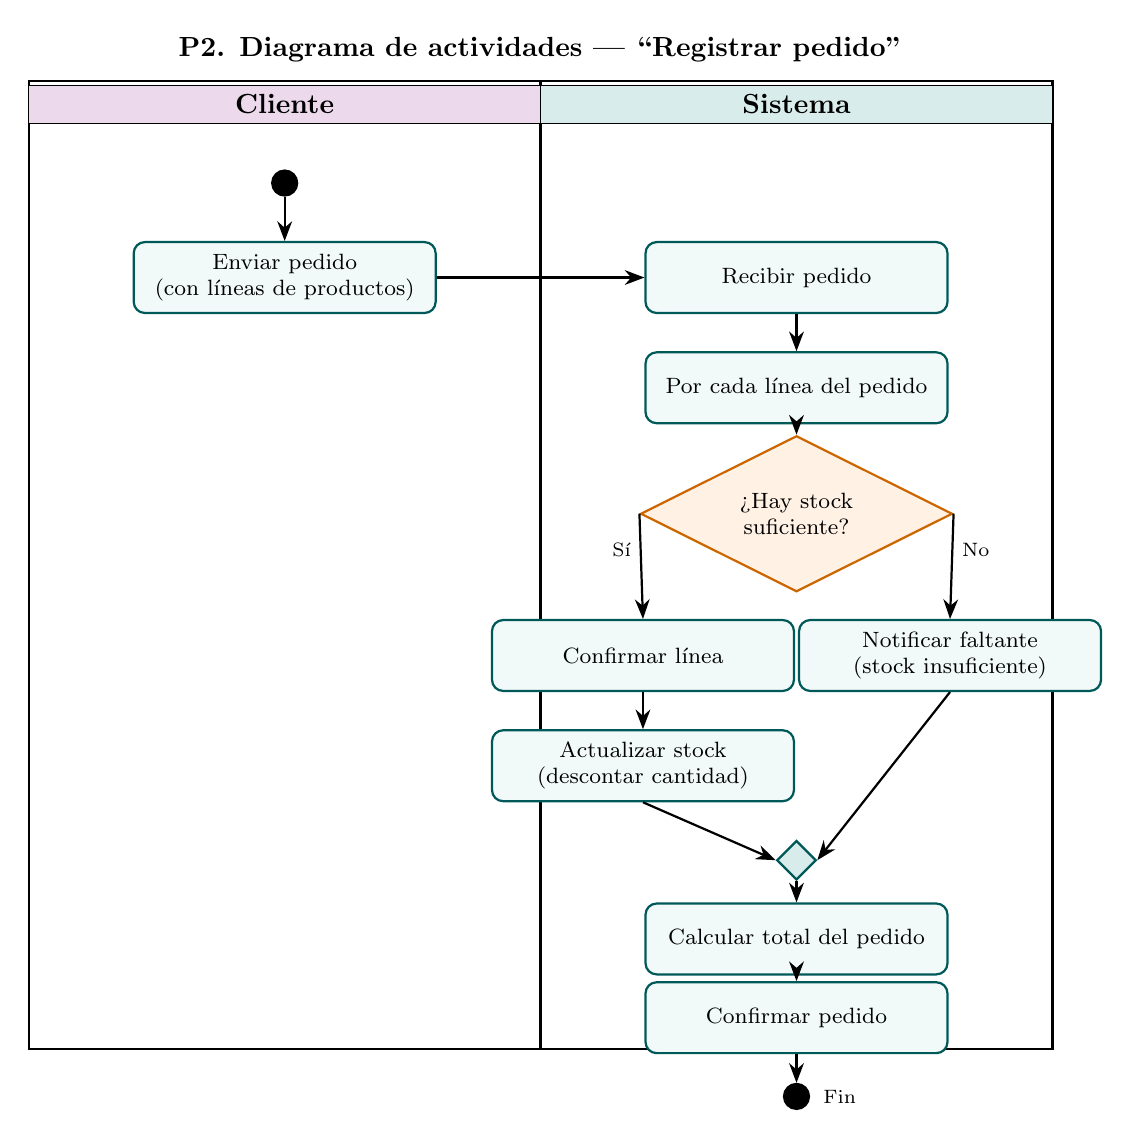
\begin{tikzpicture}[
    action/.style={rectangle, rounded corners, draw=teal!70!black, thick,
        fill=teal!5, text width=3.6cm, align=center, minimum height=0.9cm, font=\footnotesize},
    decision/.style={diamond, draw=orange!80!black, thick, fill=orange!10,
        aspect=2, text width=2.2cm, align=center, font=\footnotesize},
    merge/.style={diamond, draw=teal!70!black, thick, fill=teal!15,
        minimum width=0.5cm, minimum height=0.5cm},
    initial/.style={circle, draw=black, fill=black, minimum size=0.3cm},
    final/.style={circle, draw=black, fill=white, minimum size=0.4cm},
    finaldot/.style={circle, draw=black, fill=black, minimum size=0.2cm},
    swimlane/.style={draw=black, thick, minimum width=6.5cm},
    every edge/.style={draw, -{Stealth[length=2.5mm]}, thick},
    lbl/.style={font=\scriptsize}
]

% --- Título ---
\node[font=\bfseries] at (6.5,12.7) {P2. Diagrama de actividades --- ``Registrar pedido''};

% --- Carriles (swimlanes) ---
\draw[thick] (0,0) rectangle (6.5,12.3);
\draw[thick] (6.5,0) rectangle (13,12.3);
\draw[very thick] (6.5,0) -- (6.5,12.3);

\node[font=\bfseries, fill=violet!15, minimum width=6.5cm, draw] at (3.25,12) {Cliente};
\node[font=\bfseries, fill=teal!15, minimum width=6.5cm, draw] at (9.75,12) {Sistema};

% --- Carril Cliente ---
\node[initial] (ini) at (3.25,11) {};
\node[action] (enviar) at (3.25,9.8) {Enviar pedido\\(con líneas de productos)};

% --- Carril Sistema ---
\node[action] (recibir) at (9.75,9.8) {Recibir pedido};
\node[action] (porcada) at (9.75,8.4) {Por cada línea del pedido};
\node[decision] (hay) at (9.75,6.8) {¿Hay stock suficiente?};

\node[action] (confirmarLinea) at (7.8,5.0) {Confirmar línea};
\node[action] (notificar) at (11.7,5.0) {Notificar faltante\\(stock insuficiente)};

\node[action] (actualizar) at (7.8,3.6) {Actualizar stock\\(descontar cantidad)};

\node[merge] (union) at (9.75,2.4) {};

\node[action] (total) at (9.75,1.4) {Calcular total del pedido};
\node[action] (confirmarPedido) at (9.75,0.4) {Confirmar pedido};

\node[finaldot] (fin) at (9.75,-0.6) {};
\node[lbl] at (10.3,-0.6) {Fin};

% --- Flujo Cliente -> Sistema ---
\draw[-{Stealth[length=2.5mm]}, thick] (ini) -- (enviar);
\draw[-{Stealth[length=2.5mm]}, thick] (enviar.east) -- (recibir.west);

% --- Flujo Sistema ---
\draw[-{Stealth[length=2.5mm]}, thick] (recibir) -- (porcada);
\draw[-{Stealth[length=2.5mm]}, thick] (porcada) -- (hay);

\draw[-{Stealth[length=2.5mm]}, thick] (hay.west) -- (confirmarLinea.north) node[lbl, midway, above left] {Sí};
\draw[-{Stealth[length=2.5mm]}, thick] (hay.east) -- (notificar.north) node[lbl, midway, above right] {No};

\draw[-{Stealth[length=2.5mm]}, thick] (confirmarLinea) -- (actualizar);
\draw[-{Stealth[length=2.5mm]}, thick] (actualizar.south) -- (union.west);
\draw[-{Stealth[length=2.5mm]}, thick] (notificar.south) -- (union.east);

\draw[-{Stealth[length=2.5mm]}, thick] (union) -- (total);
\draw[-{Stealth[length=2.5mm]}, thick] (total) -- (confirmarPedido);
\draw[-{Stealth[length=2.5mm]}, thick] (confirmarPedido) -- (fin);

\end{tikzpicture}
\end{document}

% ============================================================

\documentclass[tikz,border=10pt]{standalone}
\usepackage{tikz}
\usetikzlibrary{shapes.geometric, positioning, arrows.meta}

\begin{document}
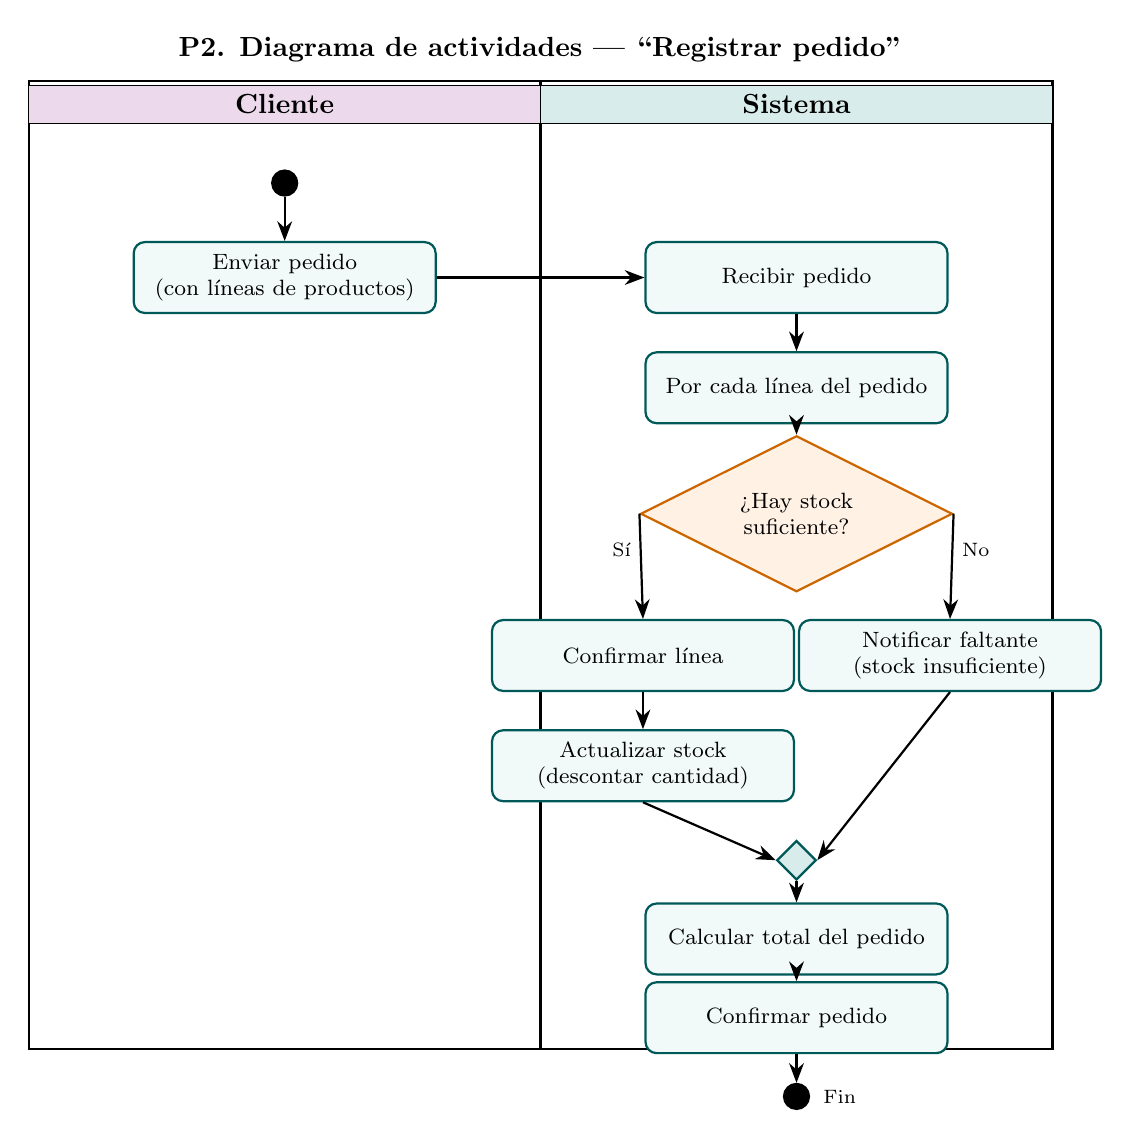
\begin{tikzpicture}[
    action/.style={rectangle, rounded corners, draw=teal!70!black, thick,
        fill=teal!5, text width=3.6cm, align=center, minimum height=0.9cm, font=\footnotesize},
    decision/.style={diamond, draw=orange!80!black, thick, fill=orange!10,
        aspect=2, text width=2.2cm, align=center, font=\footnotesize},
    merge/.style={diamond, draw=teal!70!black, thick, fill=teal!15,
        minimum width=0.5cm, minimum height=0.5cm},
    initial/.style={circle, draw=black, fill=black, minimum size=0.3cm},
    final/.style={circle, draw=black, fill=white, minimum size=0.4cm},
    finaldot/.style={circle, draw=black, fill=black, minimum size=0.2cm},
    swimlane/.style={draw=black, thick, minimum width=6.5cm},
    every edge/.style={draw, -{Stealth[length=2.5mm]}, thick},
    lbl/.style={font=\scriptsize}
]

% --- Título ---
\node[font=\bfseries] at (6.5,12.7) {P2. Diagrama de actividades --- ``Registrar pedido''};

% --- Carriles (swimlanes) ---
\draw[thick] (0,0) rectangle (6.5,12.3);
\draw[thick] (6.5,0) rectangle (13,12.3);
\draw[very thick] (6.5,0) -- (6.5,12.3);

\node[font=\bfseries, fill=violet!15, minimum width=6.5cm, draw] at (3.25,12) {Cliente};
\node[font=\bfseries, fill=teal!15, minimum width=6.5cm, draw] at (9.75,12) {Sistema};

% --- Carril Cliente ---
\node[initial] (ini) at (3.25,11) {};
\node[action] (enviar) at (3.25,9.8) {Enviar pedido\\(con líneas de productos)};

% --- Carril Sistema ---
\node[action] (recibir) at (9.75,9.8) {Recibir pedido};
\node[action] (porcada) at (9.75,8.4) {Por cada línea del pedido};
\node[decision] (hay) at (9.75,6.8) {¿Hay stock suficiente?};

\node[action] (confirmarLinea) at (7.8,5.0) {Confirmar línea};
\node[action] (notificar) at (11.7,5.0) {Notificar faltante\\(stock insuficiente)};

\node[action] (actualizar) at (7.8,3.6) {Actualizar stock\\(descontar cantidad)};

\node[merge] (union) at (9.75,2.4) {};

\node[action] (total) at (9.75,1.4) {Calcular total del pedido};
\node[action] (confirmarPedido) at (9.75,0.4) {Confirmar pedido};

\node[finaldot] (fin) at (9.75,-0.6) {};
\node[lbl] at (10.3,-0.6) {Fin};

% --- Flujo Cliente -> Sistema ---
\draw[-{Stealth[length=2.5mm]}, thick] (ini) -- (enviar);
\draw[-{Stealth[length=2.5mm]}, thick] (enviar.east) -- (recibir.west);

% --- Flujo Sistema ---
\draw[-{Stealth[length=2.5mm]}, thick] (recibir) -- (porcada);
\draw[-{Stealth[length=2.5mm]}, thick] (porcada) -- (hay);

\draw[-{Stealth[length=2.5mm]}, thick] (hay.west) -- (confirmarLinea.north) node[lbl, midway, above left] {Sí};
\draw[-{Stealth[length=2.5mm]}, thick] (hay.east) -- (notificar.north) node[lbl, midway, above right] {No};

\draw[-{Stealth[length=2.5mm]}, thick] (confirmarLinea) -- (actualizar);
\draw[-{Stealth[length=2.5mm]}, thick] (actualizar.south) -- (union.west);
\draw[-{Stealth[length=2.5mm]}, thick] (notificar.south) -- (union.east);

\draw[-{Stealth[length=2.5mm]}, thick] (union) -- (total);
\draw[-{Stealth[length=2.5mm]}, thick] (total) -- (confirmarPedido);
\draw[-{Stealth[length=2.5mm]}, thick] (confirmarPedido) -- (fin);

\end{tikzpicture}
\end{document}

% ============================================================

\documentclass[tikz,border=10pt]{standalone}
\usepackage{tikz}
\usetikzlibrary{shapes.geometric, positioning, arrows.meta}

\begin{document}
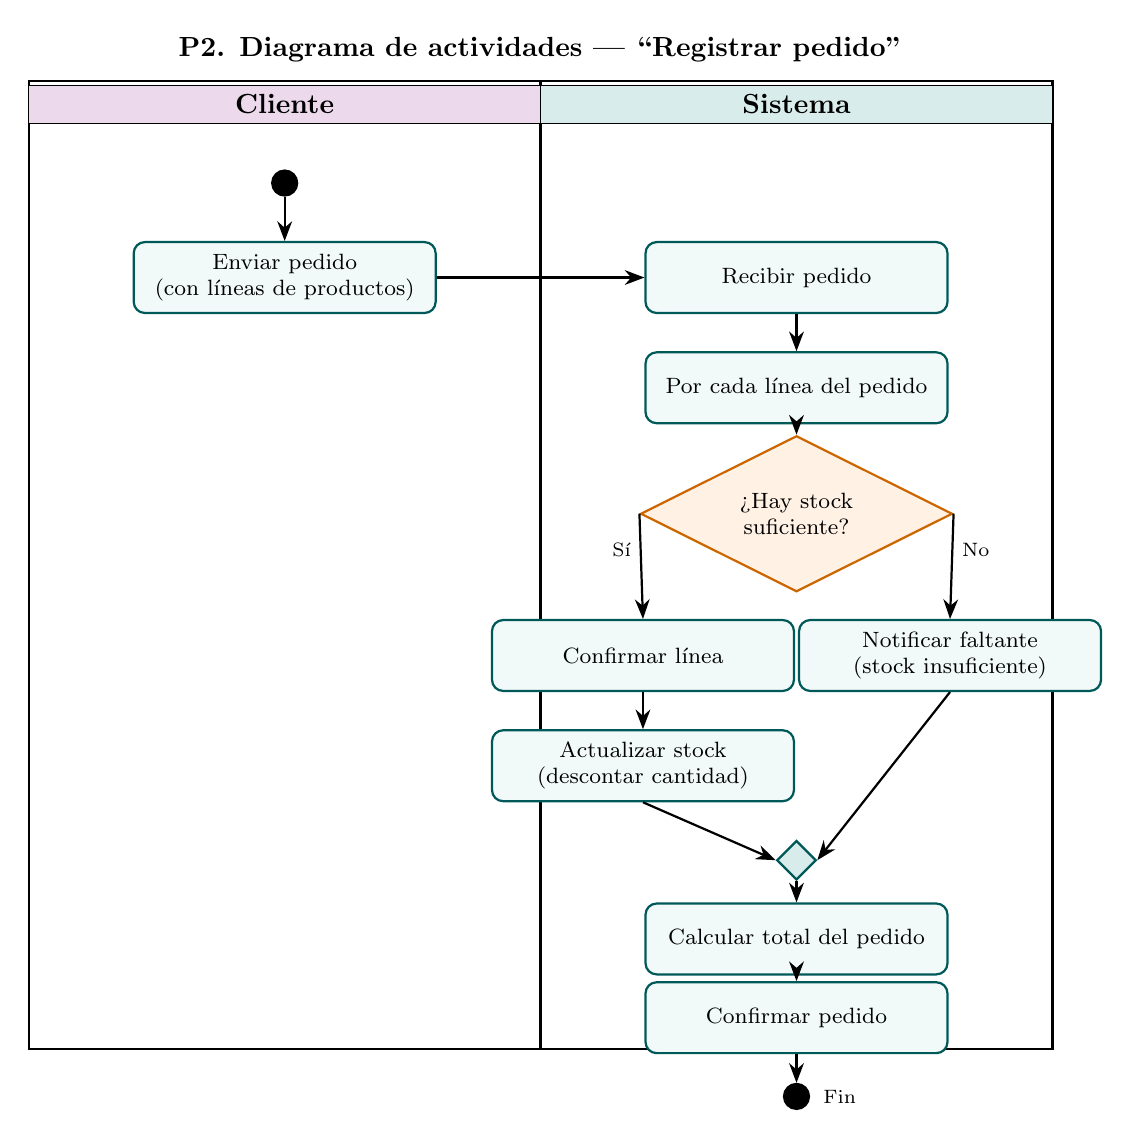
\begin{tikzpicture}[
    action/.style={rectangle, rounded corners, draw=teal!70!black, thick,
        fill=teal!5, text width=3.6cm, align=center, minimum height=0.9cm, font=\footnotesize},
    decision/.style={diamond, draw=orange!80!black, thick, fill=orange!10,
        aspect=2, text width=2.2cm, align=center, font=\footnotesize},
    merge/.style={diamond, draw=teal!70!black, thick, fill=teal!15,
        minimum width=0.5cm, minimum height=0.5cm},
    initial/.style={circle, draw=black, fill=black, minimum size=0.3cm},
    final/.style={circle, draw=black, fill=white, minimum size=0.4cm},
    finaldot/.style={circle, draw=black, fill=black, minimum size=0.2cm},
    swimlane/.style={draw=black, thick, minimum width=6.5cm},
    every edge/.style={draw, -{Stealth[length=2.5mm]}, thick},
    lbl/.style={font=\scriptsize}
]

% --- Título ---
\node[font=\bfseries] at (6.5,12.7) {P2. Diagrama de actividades --- ``Registrar pedido''};

% --- Carriles (swimlanes) ---
\draw[thick] (0,0) rectangle (6.5,12.3);
\draw[thick] (6.5,0) rectangle (13,12.3);
\draw[very thick] (6.5,0) -- (6.5,12.3);

\node[font=\bfseries, fill=violet!15, minimum width=6.5cm, draw] at (3.25,12) {Cliente};
\node[font=\bfseries, fill=teal!15, minimum width=6.5cm, draw] at (9.75,12) {Sistema};

% --- Carril Cliente ---
\node[initial] (ini) at (3.25,11) {};
\node[action] (enviar) at (3.25,9.8) {Enviar pedido\\(con líneas de productos)};

% --- Carril Sistema ---
\node[action] (recibir) at (9.75,9.8) {Recibir pedido};
\node[action] (porcada) at (9.75,8.4) {Por cada línea del pedido};
\node[decision] (hay) at (9.75,6.8) {¿Hay stock suficiente?};

\node[action] (confirmarLinea) at (7.8,5.0) {Confirmar línea};
\node[action] (notificar) at (11.7,5.0) {Notificar faltante\\(stock insuficiente)};

\node[action] (actualizar) at (7.8,3.6) {Actualizar stock\\(descontar cantidad)};

\node[merge] (union) at (9.75,2.4) {};

\node[action] (total) at (9.75,1.4) {Calcular total del pedido};
\node[action] (confirmarPedido) at (9.75,0.4) {Confirmar pedido};

\node[finaldot] (fin) at (9.75,-0.6) {};
\node[lbl] at (10.3,-0.6) {Fin};

% --- Flujo Cliente -> Sistema ---
\draw[-{Stealth[length=2.5mm]}, thick] (ini) -- (enviar);
\draw[-{Stealth[length=2.5mm]}, thick] (enviar.east) -- (recibir.west);

% --- Flujo Sistema ---
\draw[-{Stealth[length=2.5mm]}, thick] (recibir) -- (porcada);
\draw[-{Stealth[length=2.5mm]}, thick] (porcada) -- (hay);

\draw[-{Stealth[length=2.5mm]}, thick] (hay.west) -- (confirmarLinea.north) node[lbl, midway, above left] {Sí};
\draw[-{Stealth[length=2.5mm]}, thick] (hay.east) -- (notificar.north) node[lbl, midway, above right] {No};

\draw[-{Stealth[length=2.5mm]}, thick] (confirmarLinea) -- (actualizar);
\draw[-{Stealth[length=2.5mm]}, thick] (actualizar.south) -- (union.west);
\draw[-{Stealth[length=2.5mm]}, thick] (notificar.south) -- (union.east);

\draw[-{Stealth[length=2.5mm]}, thick] (union) -- (total);
\draw[-{Stealth[length=2.5mm]}, thick] (total) -- (confirmarPedido);
\draw[-{Stealth[length=2.5mm]}, thick] (confirmarPedido) -- (fin);

\end{tikzpicture}
\end{document}
